\documentclass[]{article}
\usepackage{geometry}
\geometry{margin=1in}
%opening
\usepackage{booktabs}
\usepackage[scale=2]{ccicons}

\usepackage{graphicx}
\graphicspath{Photos/}
\usepackage{amsmath,amsfonts,amssymb}
\usepackage{listings}
\usepackage{xcolor}   % for \textcolor
\usepackage{hyperref}
%opening
\title{Failure Analysis of a 1/4" Ball Valve}
\author{Ghulam Haider, Daniel Moses}

\begin{document}

\maketitle

\begin{abstract}
	
	Premature ball valve failure can lead to many undesirable outcomes including system downtime, quality issues, and safety hazards. This project investigates the failure modes of a severely eroded 1/4" ball valve and ball valves in general. A thorough investigation of failure progression for this particular valve and its components is carried out to determine the failure chain and root cause. Finally, based on this investigation, recommendations for design improvements and best practices for application are made.
	

\end{abstract}
\tableofcontents
\pagebreak
\section{Summary of Conclusions and Recommendations}
The 1/4" ball valve from the University of Tulsa’s north campus failed due to extreme erosion, causing the valve to improperly seal and eventually leak. The primary failure mechanisms include both operational errors and fluid characteristics.

\textbf{Operational Errors:}
\begin{itemize}
	\item The valve was left partially open for a throttling application
	\item The valve was likely not tightened according to specification, resulting in insufficient seal pressure
\end{itemize}

\textbf{Fluid Characteristics}
\begin{itemize}
	\item Abrasive particle residue (sand) was found on the ball and seal surfaces. 
	\item Corrosive solvent residue (salt) was found on the ball and seal surfaces.
\end{itemize}

Ball valves are not suggested for continuous throttling operations in this environment. Alternative valve selection is recommended if future leaks and frequent valve replacement are to be avoided.

\section{Introduction}
The ball valve for this study came from the University of Tulsa's north campus. The valve application, operating conditions, and length of service life were not known at the beginning of the investigation. 


Ball valves are used to control fluid flow in a line or pipe. Ball valves are different from other types of valves, in that the valve does not impede flow when in the open position. While ball valves of varying design and complexity exist, this study will focus on simple ball valves whose components and their failure modes are generally applicable to most ball valve types.

\subsection{Ball Valve Components and Operation}




\subsection{1/4" Ball Valve Case Study}



\section{Initial Visual Inspection}
Initial visual examination revealed several obvious areas of erosion within the valve. Some of the most severe damages are highlighted in  \ref{fig:Ball Valve as Recieved} 

\begin{figure}[htbp]
	\centering
	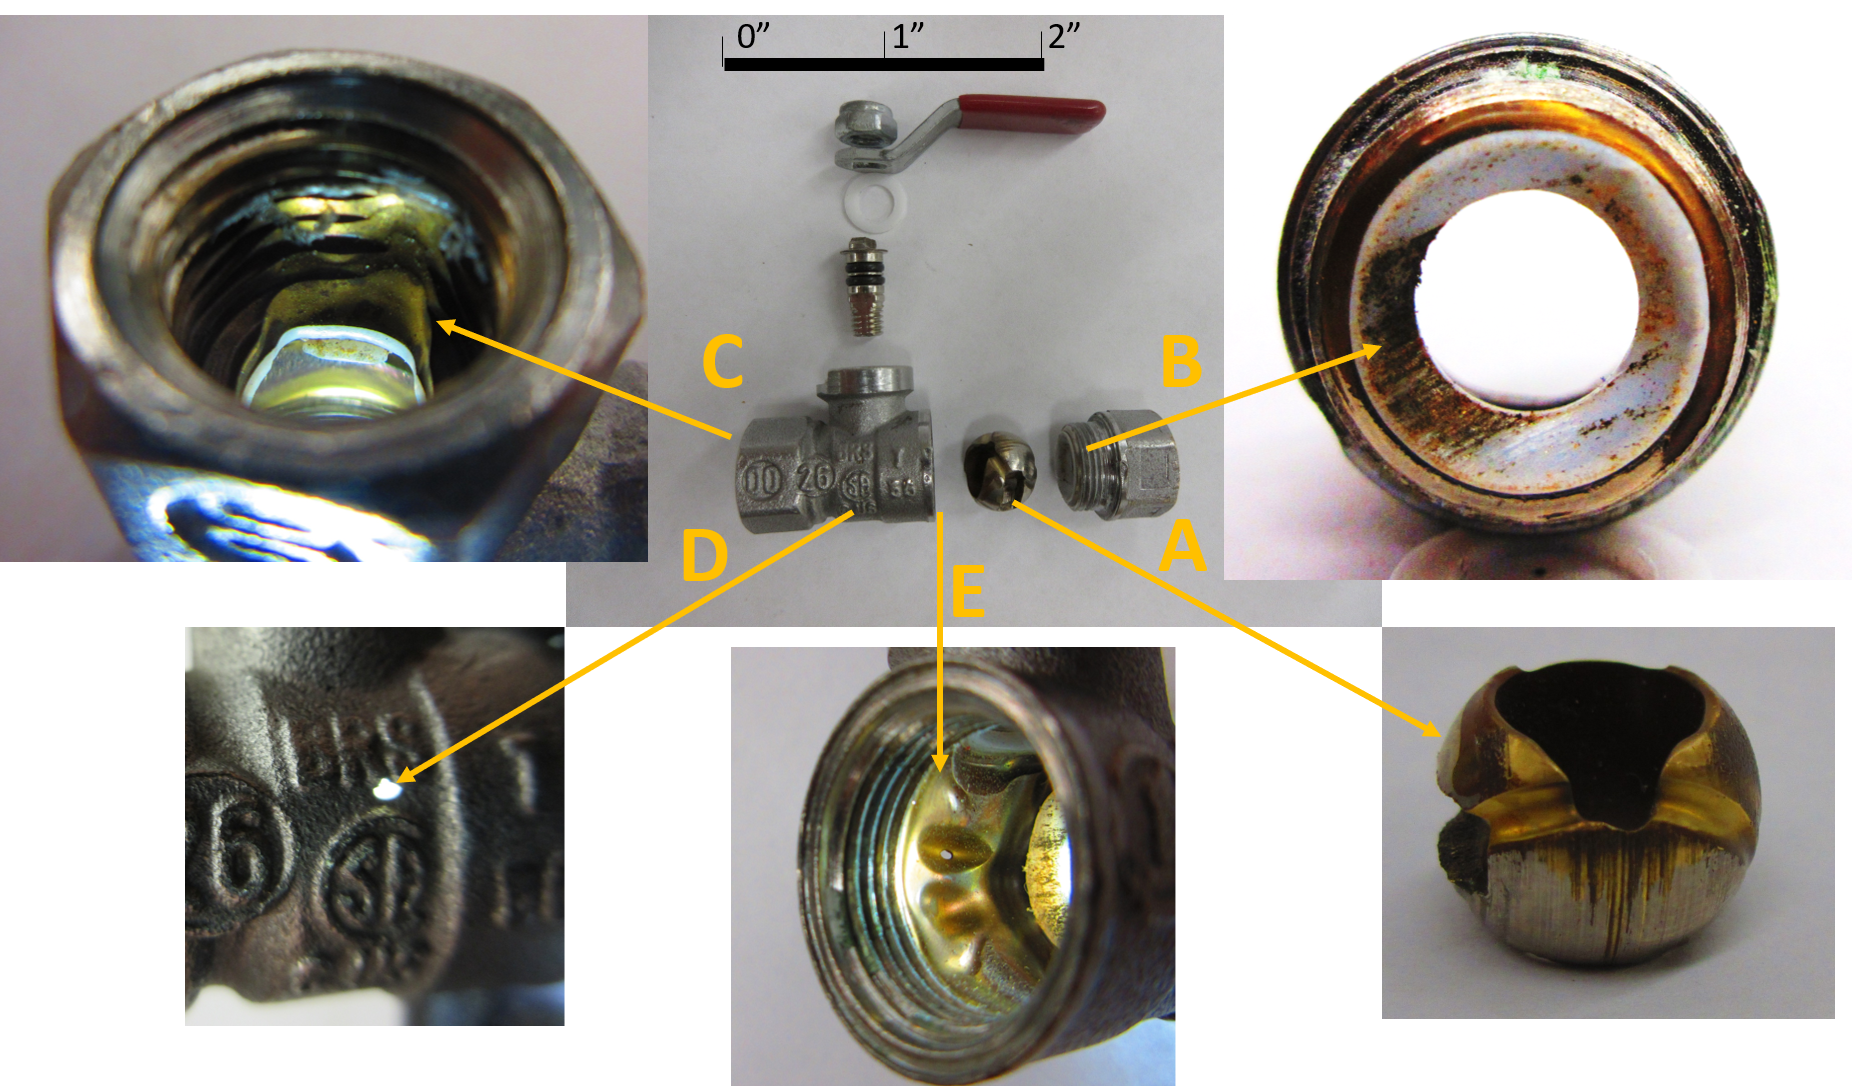
\includegraphics[width=0.9\linewidth]{Photos/Exploded_Callouts}
	\caption{A: Nickle plated brass ball; B: Nickle plated 1/4" brass nipple with Teflon seal; C: Erosion of valve body outlet; D: Pin hole outside valve body; E: Erosion of valve body inlet}
	\label{fig:Ball Valve as Recieved}
\end{figure}

\section{Laboratory Examinations}

\subsection{SEM}
Text

\begin{figure}[htbp]
	\centering
	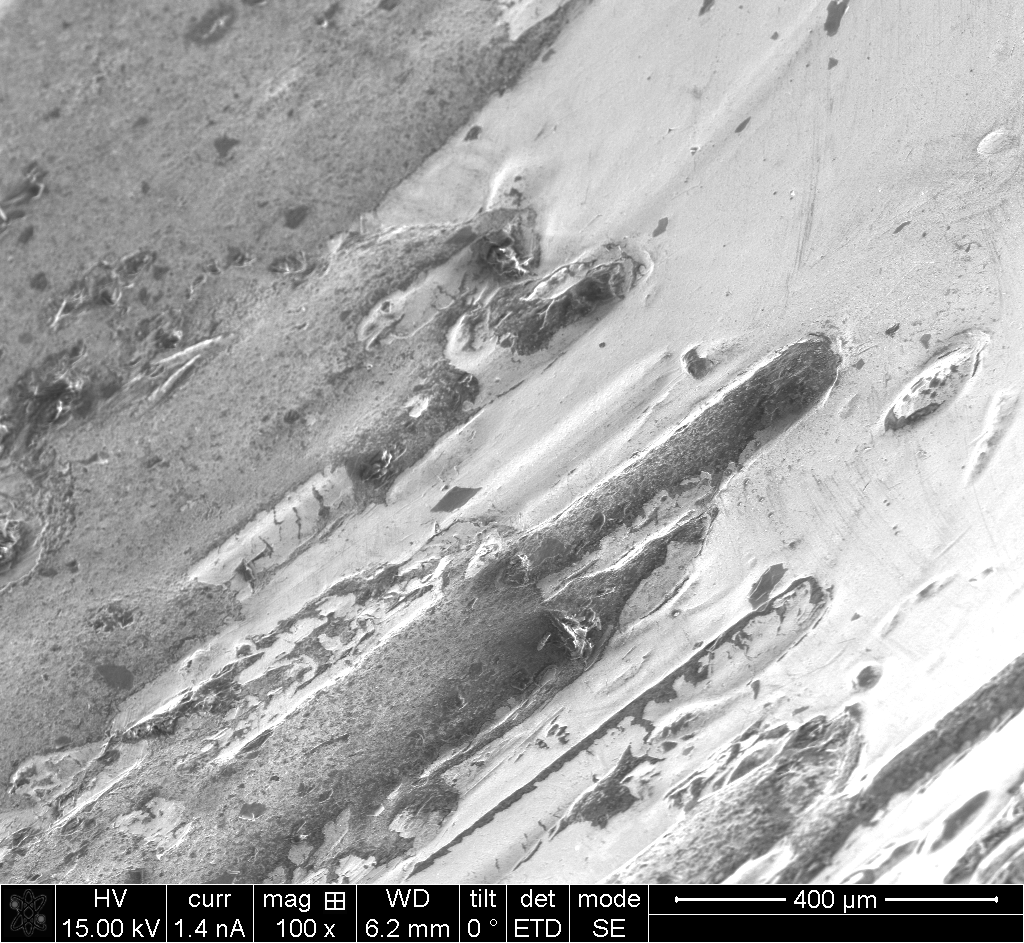
\includegraphics[width=0.8\linewidth]{Photos/SEM_01.png}
\end{figure}

more text
\subsection{Metallographic Examination}
\subsection{Seal Pressure}


\section{Analysis}
\subsection{CFD}

\section{Recommendations}
\subsection{Research Considerations}
Valve application is an import factor to consider in recommending design changes. In particular, economic and safety considerations should be included in the decision making process.

Due to the experimental nature of the system, valve configuration may not be permanent, may be economically feasible with periodic replacement in mind, recommend routine inspection. Care should be taken to install the valve with proper torque.

This model of ball valve may not be appropriate for maintaining precision flow over many tests, since the valve throttling will not remain constant as the valve is eroded. This valve may also be inappropriate for use with fluids that pose an environmental or safety hazard to researches, since the first noticeable sign of failure is fluid leaking. 

\end{document}